\begin{comment}
・OEB使用時と平面ディスプレイ使用時の2回の実験を行った(プレゼンター1人,質問者3人)

・平面ディスプレイ使用の実験の後,10分程度の休憩時間を設け,OEBを使用する実験に移った

・実験の開始前に,使用するアプリケーションの操作説明を行った

・また,5分程度,事前準備したスライドの内容をある程度覚えてもらった(プレゼン中,出来るだけ映像の方を見てもらうため)

・プレゼンターは,プレゼン中,3つ存在するプレゼン内容のチャックポイントに合わせ,ランダムな順番で1人づつ,対応する被験者を見てもらった

・また,質問中は質問を受けている被検者の方向を見るように指示した

・OEB使用時は,見る被験者の映像をクリックし続けることで,視線情報のログを取った

・平面ディスプレイ使用中は,被検者それぞれに対応したキー(映像に移っている左の人間からA,S,D)を押しっぱなしにしてもらうことで視線情報のログを取った

・一方,質問者側の被験者3人には,プレゼン中はプレゼンを聴くように指示した

・質問は,事前に準備した質問3つをランダムな順番で行った(プレゼンターから質問するように促される)

・上記の質問が終わったのちは各質問者から自由に質問してもらい,プレゼンと質問合わせて約10分使用した
\end{comment}
この節では,実験中の被験者の行動の仔細について述べる.
先述の通り,実験はOmniEyeBall使用時と平面ディスプレイ使用時の2回の実験を行った.
プレゼンターは1人で,傍聴者は3人であった.両サイドは異なる部屋で実験を行い,無線
遠隔通信でのビデオ会議を行った.2実験の間には約10分の休憩を設けた

実験の開始前に,使用するアプリケーションの説明を行った.
プレゼンターには,各傍聴者の周辺をクリックすると傍聴者が正面にくること.
及び,OmniEyeBallでどのように映像が表示されるかを伝えた.一方で
傍聴者側には,自身が見られていると全天球カメラに映ったプレゼンターが
個人の方向を向くこと,それ以外の状況では画面上部に小窓が表示されることを
伝えた.

一方で,プレゼンテーションや質問についても一定の指示を行った.
プレゼンターに対しては,プレゼンテーション前に,出来るだけ
カメラの方向を見てもらえるように,事前準備したスライドの内容を
5分ほど眺めてもらい,大筋を把握するように指示した.
また,準備した資料には3つのチェックポイントを設けて,その
部分を読み上げるタイミングで,ランダムな順番で1人毎,傍聴者を
見るように指示した.質問中は,質問を受けている傍聴者の方向を
見るように指示した.さらに,誰を見ていたかをリアルタイムで記録するために
追加の操作を行ってもらった.OmniEyeBall使用時は,見ている傍聴者の
映像をクリックし続けるように,平面ディスプレイ使用時は,傍聴者それぞれに
対応したキーボードのキーを押し続けてもらうことで視線情報の履歴を
録った.

傍聴者側には,タブレット端末を渡し,
プレゼンターの紹介するプレゼン資料を事前に
配布し,プレゼンテーション中にいつでも参照できるようにした.
プレゼンターのプレゼンテーション中には,資料を好きに参照しながら
傍聴してもらうように指示した.質疑応答の時間には,事前準備した
質問3つをランダムな順番で1人1つづつ問うようにしてもらい,その後は
自由に質問するように指示した.定量的評価のため,プレゼンターを目が
合ったと感じている間は,指定のキーを押し続けてもらうように指示した.

\begin{figure}[tp]
    \centering
    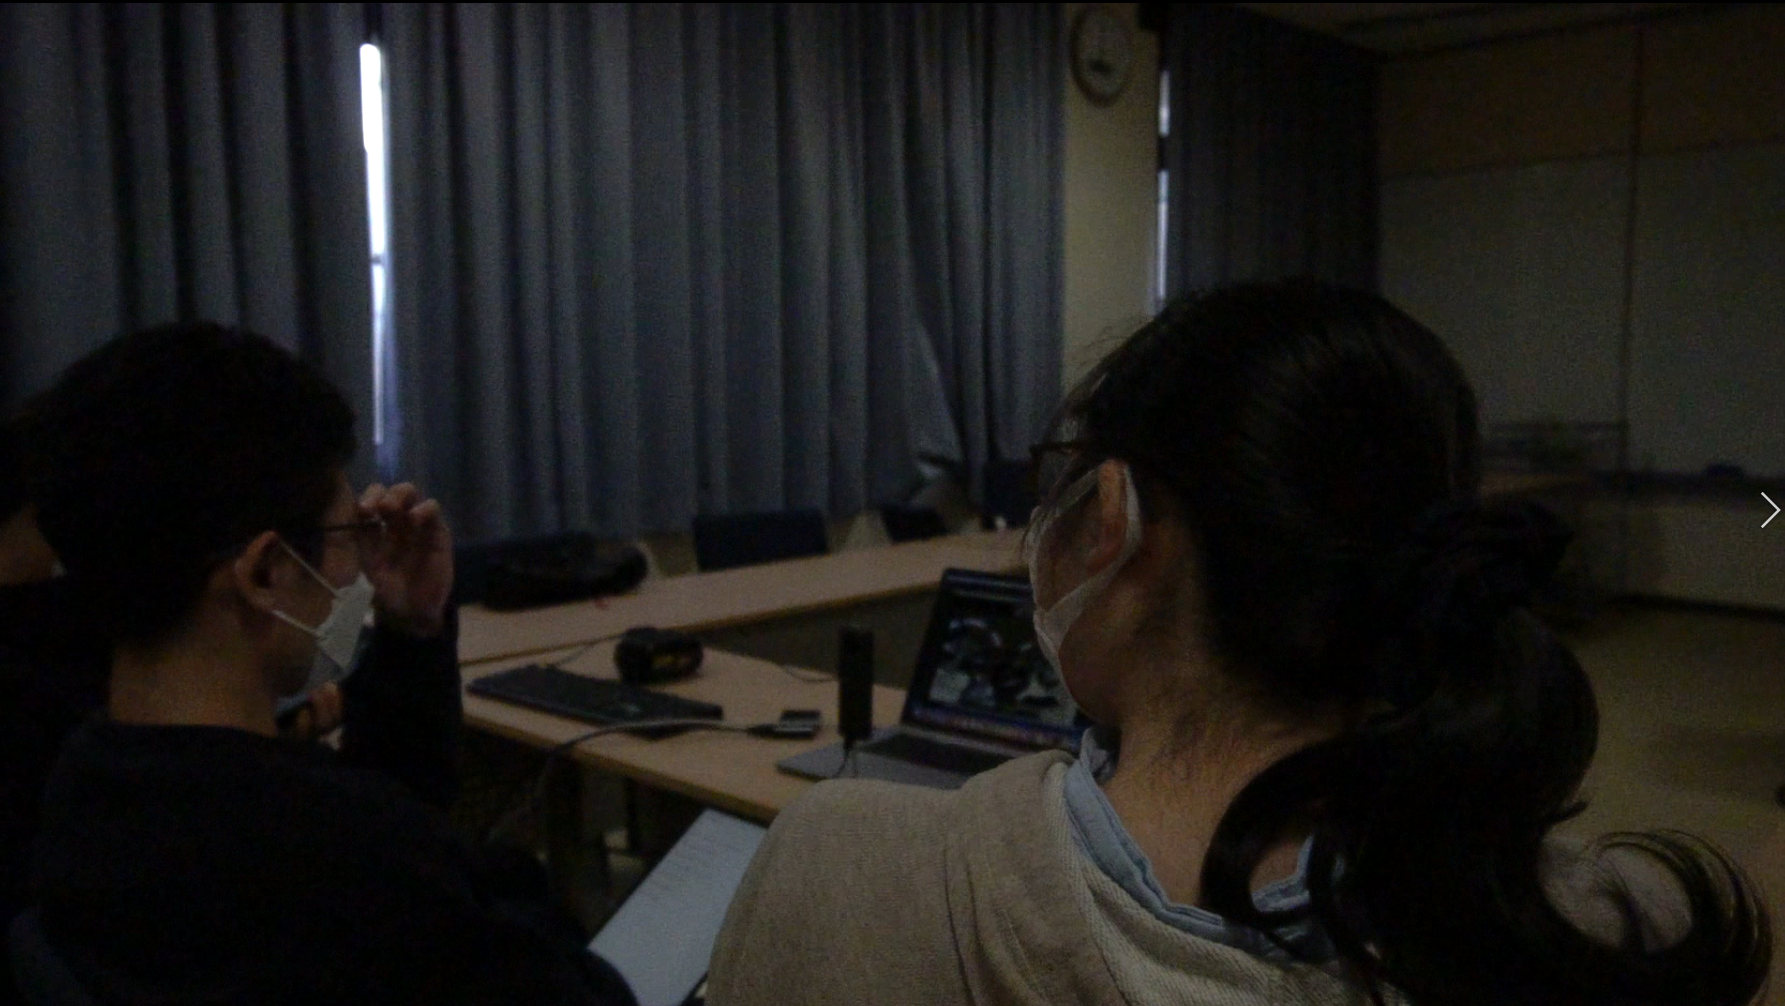
\includegraphics[scale=0.4]{fig/exp1.png}
    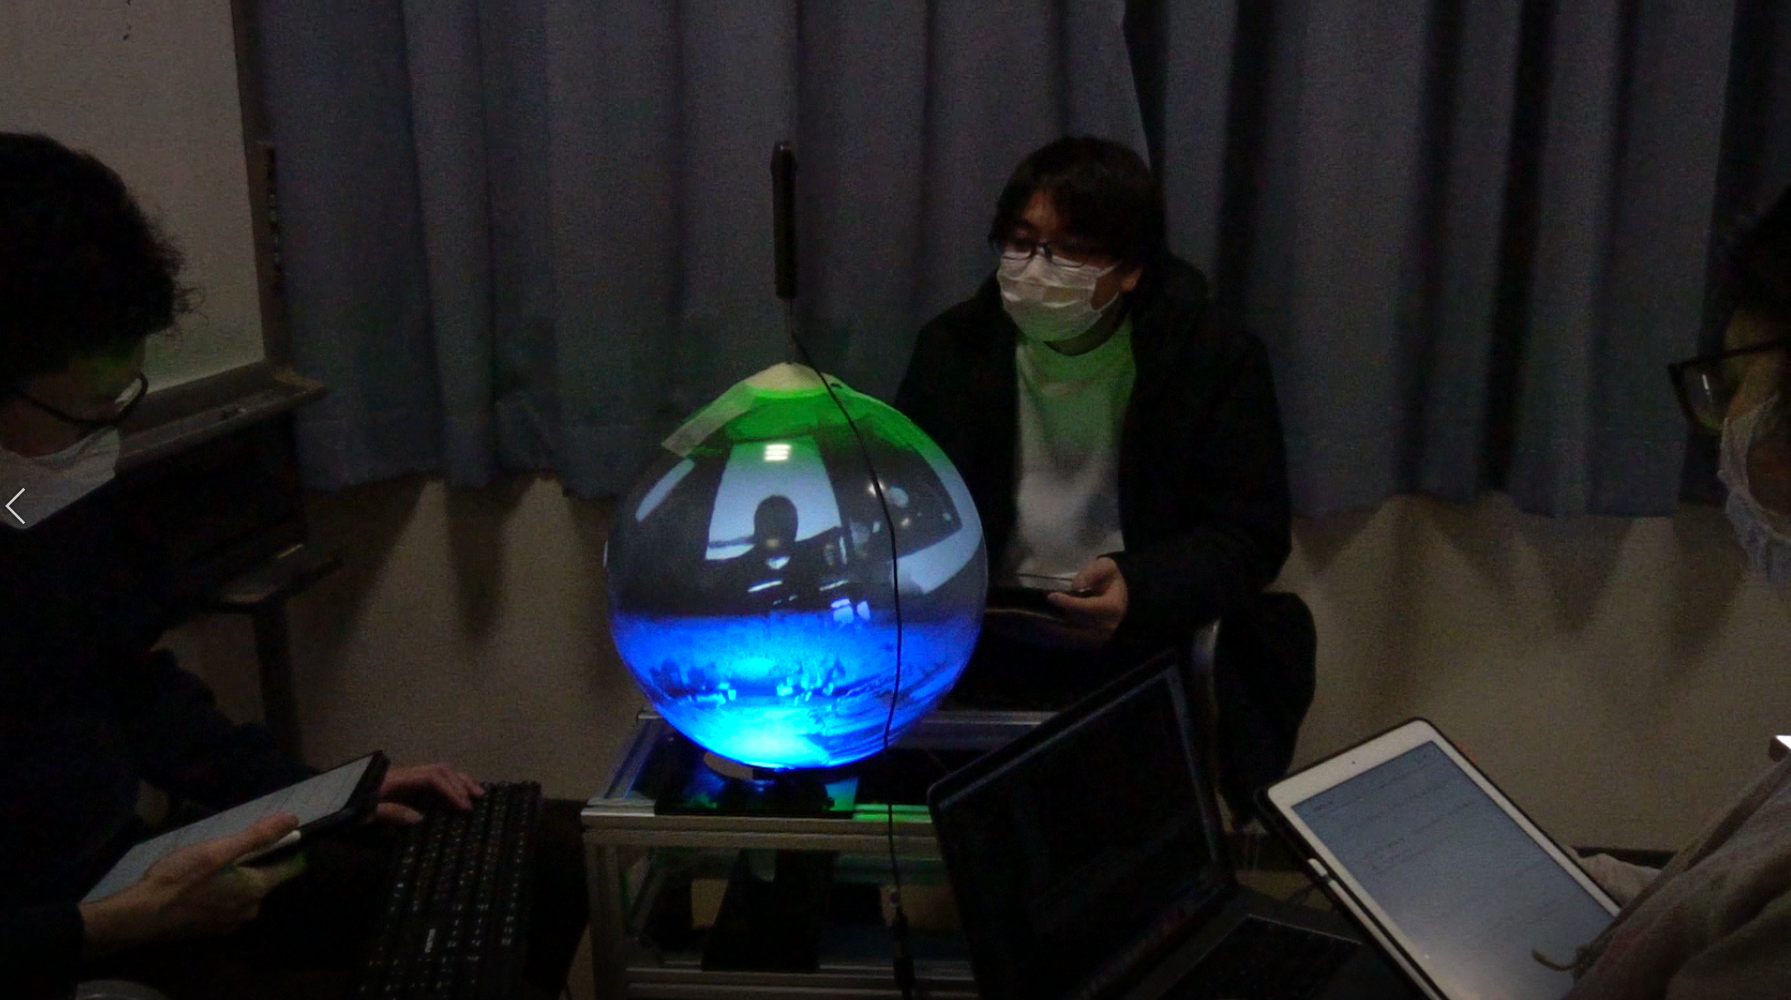
\includegraphics[scale=0.4]{fig/exp2.png}
    \caption{傍聴者側の実験の様子}
\end{figure}

\begin{figure}[tp]
    \centering
    \includegraphics[scale=0.3]{fig/exp4.png}
    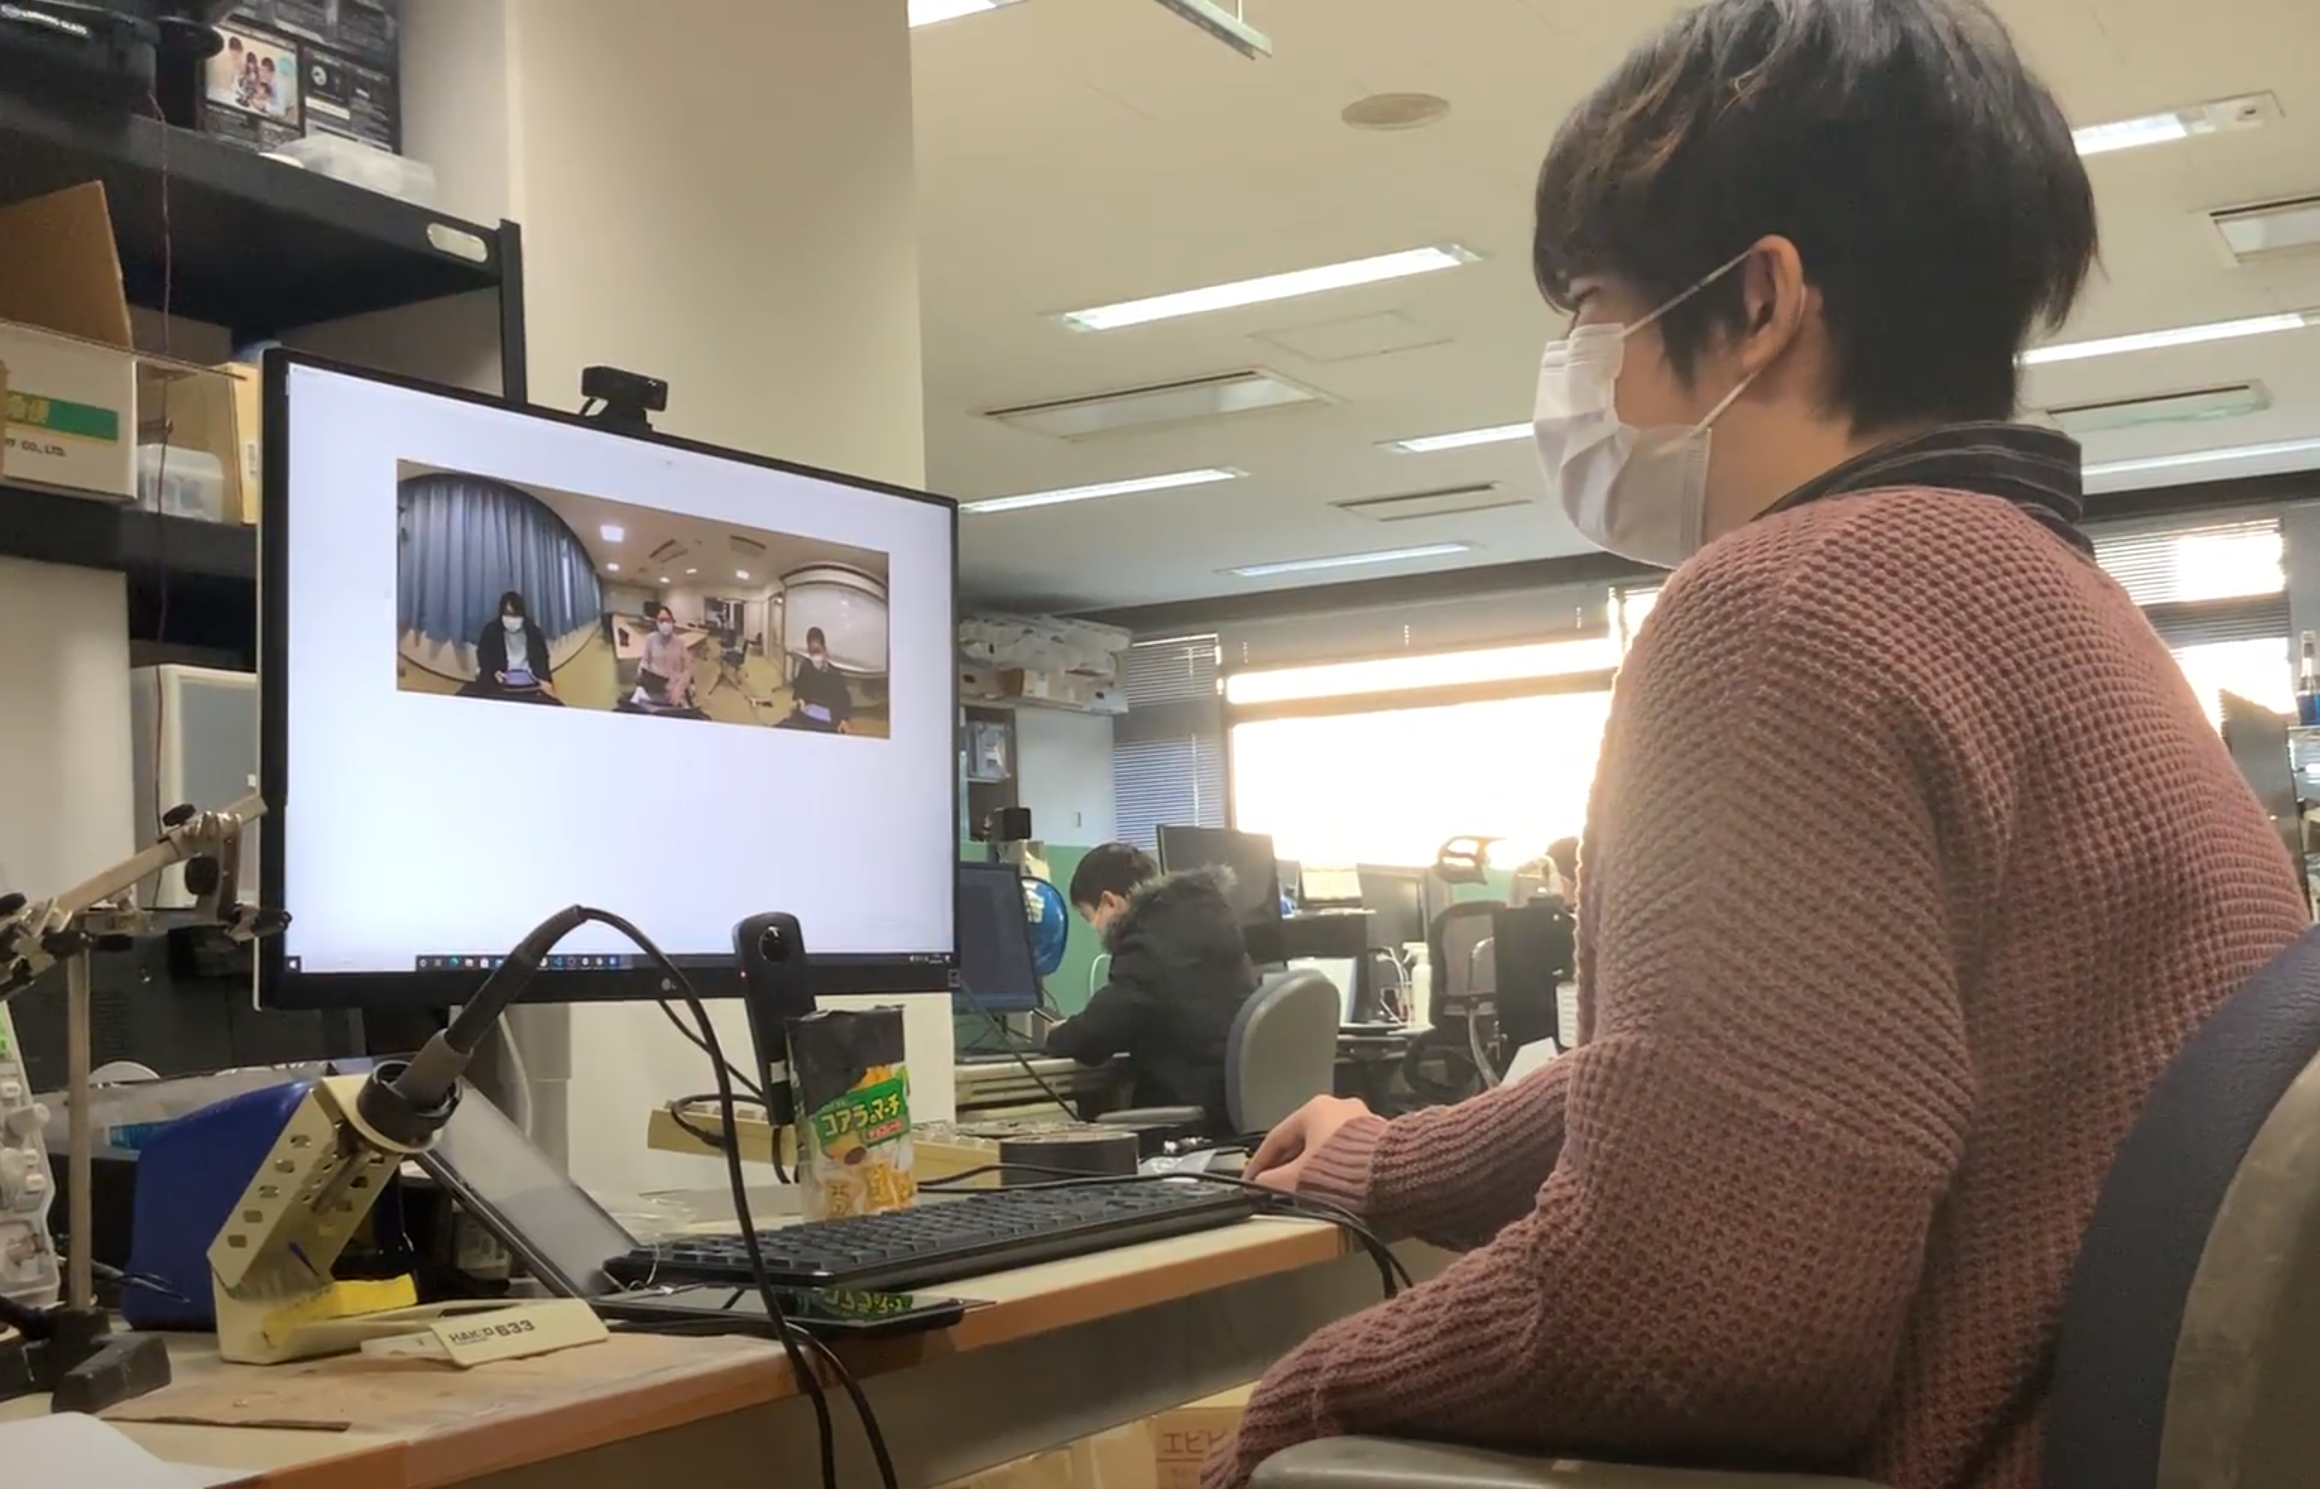
\includegraphics[scale=0.3]{fig/exp3.png}
    \caption{プレゼンター側の実験の様子}
\end{figure}